%In this section, we introduce GraphFlow. \cite{shen2023towards}


\subsection{KG-based RAG as Multi-step Decision}
\xhdr{Problem Formulation}
Given an input query $\mathcal{Q}$, our goal is to retrieve a set of $K$ target nodes $\mathbb{V}^{*}=\{V_{i} \mid i=1,\cdots,K\}$ from a text-rich knowledge graph (KG) $\mathcal{G} = \{\mathbb{V}, \mathbb{E}, \mathbb{D}\}$ such that the associated documents $\mathbb{D}^{*} = \{D^{*}_{i} \mid i=1,\cdots,K\}$ can support answering $\mathcal{Q}$. Here, $V_{i} \in \mathbb{V}$ is a node, $E_{ij} \in \mathbb{E}$ is an edge between $V_{i}$ and $V_{j}$ indicating their relation. Each $D_{i}$ denotes the textual document associated with node $V_{i}$ (e.g., the content of a paper).


\xhdr{Agent-based Retrieval as a Multi-step Decision Process}
    To effectively leverage both relational and text information in the KG, we employ the agent-based approach initiated with an LLM due to its superior text understanding and planning ability. 
    %We model agent-based retrieval as a multi-step decision problem with the following components:
    We formulate the agent-based retrieval as a multi-step decision problem, consisting of the following components:
\begin{itemize}
    \item \textbf{State.} The agent starts retrieval from the initial state $s_{0} = (\mathcal{Q}, \{D_{0}\})$, where $D_{0}$ is the document associated with the source node $V_{0}$ from which the retrieval process is initiated. 
    At step $t$, the agent arrives at node $V_{t}$ and the current state is defined as $s_{t} = (\mathcal{Q}, \{D_{j}\}_{j=0}^{t})$, where $\{D_{j}\}_{j=0}^{t}$ is the set of documents collected along the partial retrieval trajectory $\tau_{\leq t} = V_{0} \rightarrow \cdots \rightarrow V_{t}$.
    \item \textbf{Action.} Given state $s_{t}$, the agent selects an action $a_{t} \in \mathcal{A}(s_{t})$, corresponding to moving from $V_{t}$ to a adjacent node $V_{t+1} \in \mathrm{N}(V_{t})$ along edge $E_{t,t+1}$.
    The agent then retrieves the documents $D_{t+1}$ associated with $V_{t+1}$.
    \item \textbf{Transition.} The agent transits to state $s_{t+1}=(\mathcal{Q}, \{D_{j}\}_{j=0}^{t+1})$. 
    This process continues until either the document $D_{t+1}$ is deemed sufficient to support the query $\mathcal{Q}$, or a predefined maximum number of steps is reached.
    \item \textbf{Reward.} Upon termination, the agent receives a reward $R(\tau)$ for the retrieval trajectory $\tau$. The reward is calculated whether the document $D_{\mathrm{T}}$ associated with the terminal node $V_{\mathrm{T}}$ of trajectory $\tau$ can the query (i.e. $D_{\mathrm{T}}\in\mathbb{D}^{*}$).
\end{itemize}
\begin{figure}[t]
%\vspace{-0.3cm}
\begin{center}
\footnotesize
\centerline{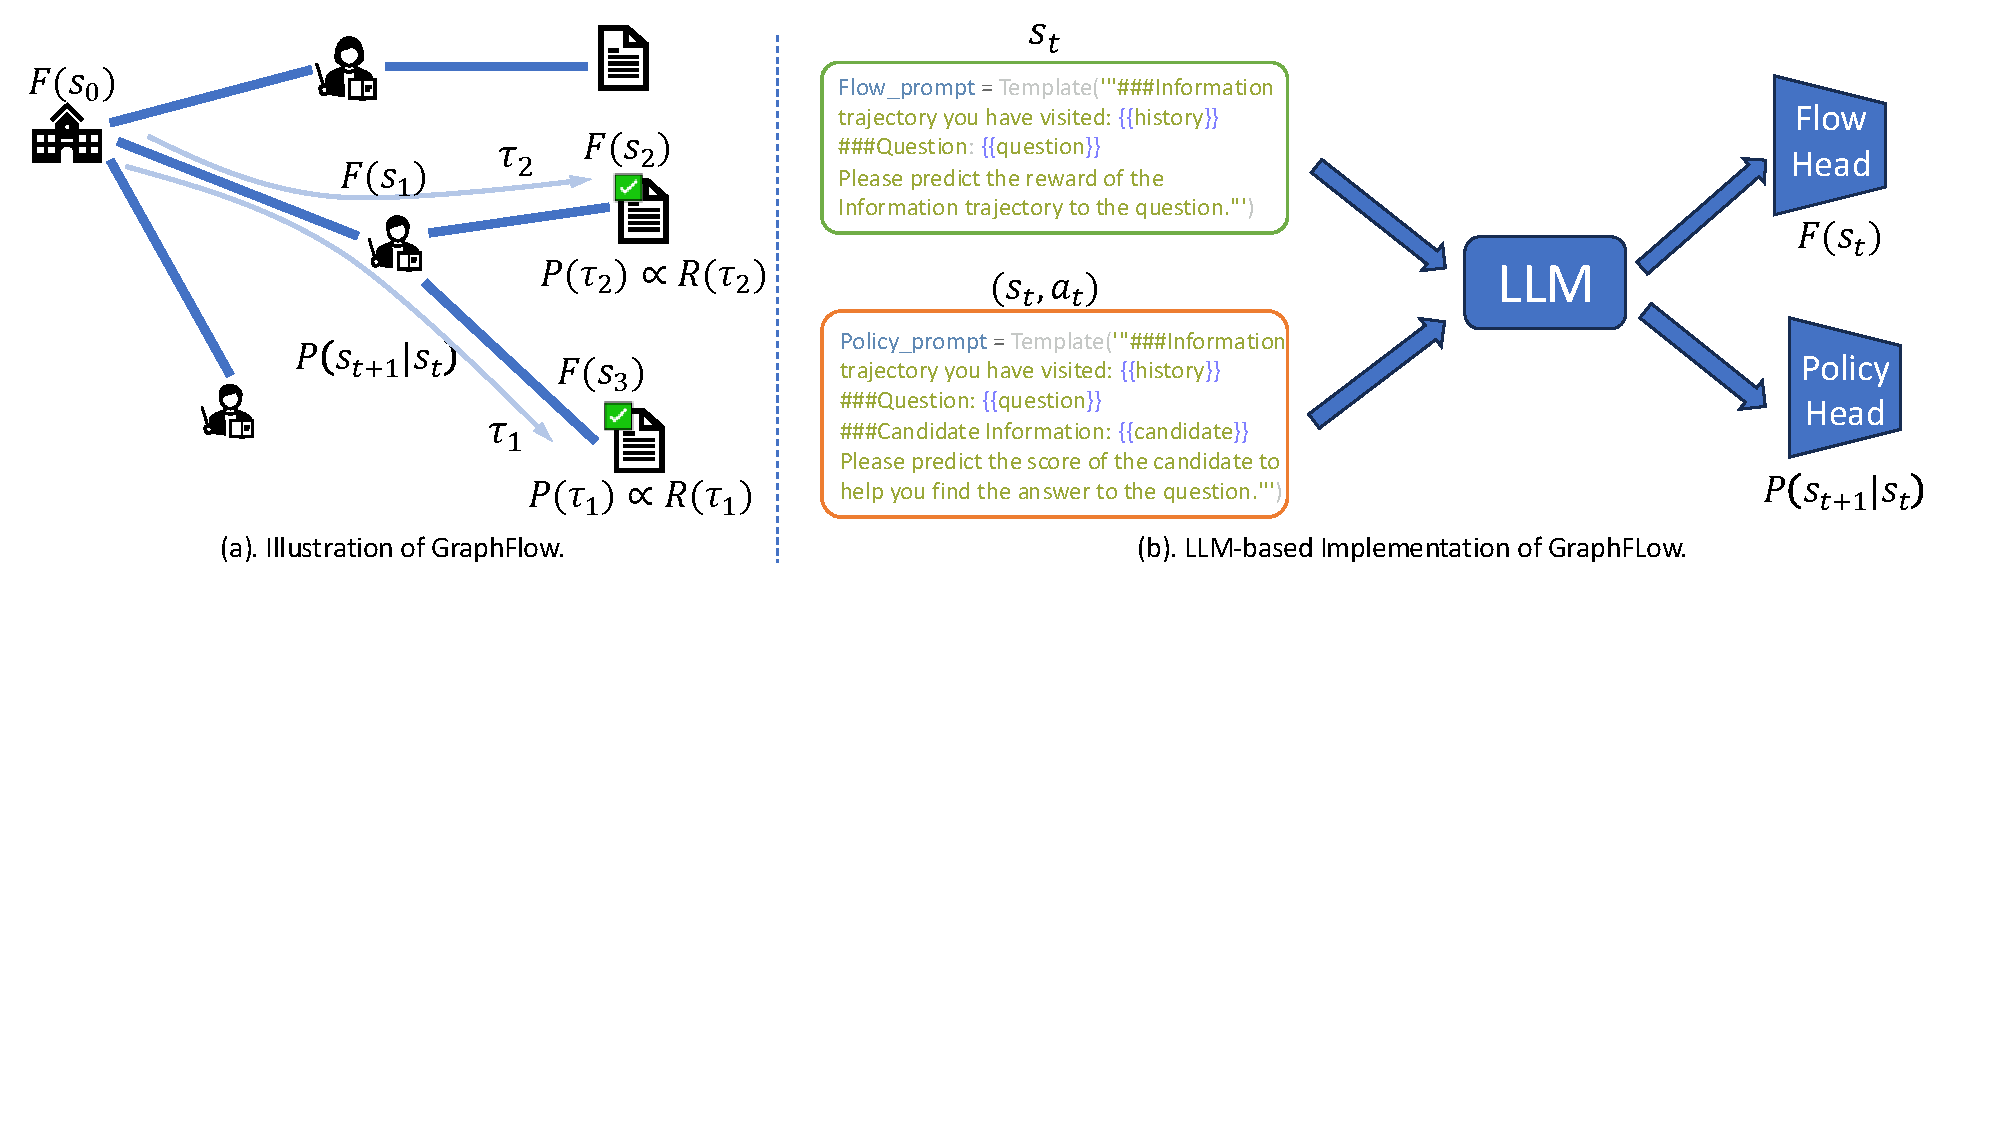
\includegraphics[width=0.85\columnwidth]{flowchart.pdf}}
\end{center}
\vspace{-0.8cm}
\caption{An overview of the proposed GraphFlow framework. (a). GraphFlow employs a flow estimator $F(\cdot)$ to factorize the outcome reward $R(\tau)$ of a retrieval trajectory $\tau$ to flow value $F(s_{t})$. The flow value guides to learn a policy $P(s_{t+1}|s_{t})$ that leads to accurate and diverse retrieval results for complex queries. (b) We introduce an LLM-based implementation of GraphFlow to enhance KG-based RAG on text-rich KGs.} 
\vspace{-0.5cm}
\label{figure:flowchart}
\end{figure}

\xhdr{Energy-based Modeling for Accurate and Diverse Retrieval}
As shown in Figure~\ref{figure:flowchart} (a), the goal of GraphFlow is to learn the policy $P(s_{t+1}\mid s_{t})$ that can effectively retrieve accurate and diverse information from a knowledge graph (KG) to support answering an input query. 
To this end, we formulate the retrieval process as an energy-based distribution over trajectories:
\begin{equation}
    \begin{aligned}
        P(\tau)= \prod_{t=0}^{\mathrm{T}} P(s_{t+1}\mid s_{t})\propto R(\tau).
    \end{aligned}
    \label{energy-based_obj}
\end{equation}
The equality in Eq.~\ref{energy-based_obj} is due to the Markov property of the state transition. 

In contrast to the objectives of prior KG-based RAG methods in Eq.~\ref{obj:maxize_1} and Eq.~\ref{obj:maxize_2} that maximize the likelihood of the most relevant information in KG, the objective of GraphFlow in Eq.~\ref{energy-based_obj} reflects the intuition that high-reward retrieval trajectories (i.e., trajectories ending in high-quality supporting documents) should be sampled more frequently.
Thus, GraphFlow naturally promotes diverse yet accurate retrieval results since the retrieval trajectories resulting in highly relevant documents are more likely to be explored.
Moreover, GraphFlow also enjoys good generalization ability by avoiding strict likelihood maximization and does not overfit to a few dominant candidates.


\subsection{Flow Estimation as Credit Assignment}

A major challenge in learning the policy $P(s_{t+1} \mid s_t)$ to satisfy Eq.~\ref{energy-based_obj} is the lack of process-level supervision. 
When collecting retrieval trajectories $\tau\in\mathcal{T}$ for training, only the outcome reward $R(\tau)$ is observable, indicating whether the final retrieved document supports answering the query.
Annotating the process-level reward signals for every intermediate state and action is expensive. 
This gives rise to the credit assignment problem \cite{nguyen2018credit,zhou2020learning}, which attributes the terminal reward of a trajectory back to the intermediate decisions. 
To address this, we adopt the GFlowNet framework \cite{bengio2023gflownet}, which implicitly performs credit assignment by estimating a non-negative flow value for each state.

Rather than directly maximizing the reward or value of a full trajectory, GFlowNets introduce a flow function $F(s): \mathcal{S} \rightarrow \mathbb{R}_{\ge 0}$ for each intermediate state $s$. 
The learning objective enforces a local consistency constraint between transitions, which is known as the detailed balance condition:
\begin{equation} 
F(s_t) \cdot P(s_{t+1} \mid s_t) = F(s_{t+1}) \cdot P_{\text{B}}(s_t \mid s_{t+1}),
\end{equation}
where $P(s_{t+1} \mid s_t)$ is the forward policy we want to obtain, and $P_{\text{B}}(s_t \mid s_{t+1})$ is the backward policy. 
When this condition holds for all transitions, the retrieval trajectory induced by the policy $P(s_{t+1} \mid s_t)$ satisfies the objective in Eq.~\ref{energy-based_obj}, leading to diverse and accurate retrieval results on KGs.

% While other objectives of GFlowNet, such as trajectory balance \cite{malkin2022trajectory} or subtrajectory balance \cite{madan2023learning}), can also encourage diversity, they require computing on the whole trajectory or sub-trajectory. 
% In our setting, the retrieval trajectories contain multi-hop and node documents are long. Computing objective on trajectory or subtrajectory level is impractical and cause out-of-memory. Thus, we adopt the detailed balance objective that operates on transitions between states.

While alternative GFlowNet objectives, such as trajectory balance \cite{malkin2022trajectory} or subtrajectory balance \cite{madan2023learning}, can also promote diversity, they require computation over entire trajectories or sub-trajectories. 
In KG-based RAG, the retrieval trajectory involves multi-hop transitions, and each node is associated with long documents.
These objectives are computation-intensive and often lead to out-of-memory (OOM) issues. 
To ensure scalability and efficiency, we thus adopt the detailed balance objective that operates on state transitions.
% Table generated by Excel2LaTeX from sheet 'Sheet1'
\begin{table}[t]
  \centering
  \footnotesize
  \caption{Performance of retrieval accuracy of KG-based RAG methods on STaRK benchmark. Our GraphFlow outperforms baselines with higher hit rates and MRR scores. GraphFlow also surpasses strong baselines implemented with GPT-4o on most metrics.}
  \vspace{-0.2cm}
  \setlength{\tabcolsep}{0.7mm}{
    \begin{tabular}{c|c|ccc|ccc|ccc}
    \toprule
    \multirow{2}[4]{*}{Method} & Dataset & \multicolumn{3}{c|}{STaRK-AMAZON} & \multicolumn{3}{c|}{STaRK-MAG} & \multicolumn{3}{c}{STaRK-PRIME} \\
\cmidrule{2-11}          & Metric & Hit@1 $\uparrow$ & Hit@5$\uparrow$ & MRR$\uparrow$   & Hit@1$\uparrow$ & Hit@5$\uparrow$ & MRR$\uparrow$   & Hit@1$\uparrow$ & Hit@5$\uparrow$ & MRR$\uparrow$ \\
    \midrule
    \multicolumn{1}{c|}{\multirow{3}[2]{*}{\makecell{Retrieval\\-based}}} & DenseRetriver &   6.10    & 15.85   &  10.61  & 24.44  &  40.23  & 32.41  & 5.43  & 13.07 & 8.99\\
          & G-Retriever  & 6.10 & 11.59  & 8.54  & 24.44  & 31.95 &  28.08  & 5.43 & 8.94  & 6.95 \\
          & SubgraphRAG & 8.03 & 12.43 & 9.90 & 9.30   &  25.59   &  16.11     &  4.82     &  8.00     & 6.17 \\
    \midrule
    \multicolumn{1}{c|}{\multirow{5}[1]{*}{\makecell{Agent- \\ based \\ (w/o Rerank)}}} & ToG+LLaMA3 &  4.21     &   6.16   &   5.25    &   12.0    &   14.09    &   12.67    &   21.92    &   34.0    & 26.61 \\
          & ToG+GPT4o &  \textbf{20.67}     &   41.38    &   30.90    &   23.33    &   56.67    &   36.38    &   16.67    &   39.77    & 27.02 \\
          & SFT   &  8.16     &   15.30    &   13.54    &   26.53    &   28.57    &   29.10    &   27.5    &   40.07    & 33.06 \\
          & PRM   &   20.09  &  26.25  &   	28.16     &   26.05	  &  28.0 &   28.52	   &  21.01 &  46.72& 31.25   \\
          & \textbf{GraphFlow} &  19.63&  \textbf{44.17}& 	\textbf{31.66}   & \textbf{29.32}	& \textbf{58.64}	&\textbf{41.32}	 &  \textbf{39.84}& 	\textbf{71.71}	& \textbf{54.58}    \\
    \midrule
    \multicolumn{1}{c|}{\multirow{5}[1]{*}{\makecell{Agent- \\ based \\ (Rerank)}}} & ToG+LLaMA3 &4.21     &   6.16   &   5.25    &   12.0    &   14.09    &   12.67    &   21.92    &   34.0    & 26.61 \\
          & ToG+GPT4o &27.58& 	51.72& 	39.08& 	26.67& 	56.67& 	39.65& 	\textbf{53.33}& 	63.73& 	57.78 \\
          & SFT & 12.24&	30.61	&21.54	&27.55&	44.89&	36.37&	23.75&	52.5&	35.98 \\
          & PRM  &  21.25	 & 42.50 & 	31.97 & 	27.31 & 	44.09 & 	33.69 &  22.86 & 	28.24 & 	26.94 \\
          & \textbf{GraphFlow} &  \textbf{47.85}& 	\textbf{65.03}& 	\textbf{55.49}& 	\textbf{39.09}& 	\textbf{57.51}& 	\textbf{47.82}& 	51.39& 	\textbf{72.11}& 	\textbf{61.37} \\
    \bottomrule
    \end{tabular}}%
    \vspace{-0.6cm}
  \label{tab:performance-retrieval-acc}%
\end{table}%



\xhdr{Detailed Balance with Local Exploration}
Enforcing the detailed balance condition globally across all transitions in a knowledge graph (KG) is computationally inefficient, since the vast state space makes many nodes and transitions unreachable during training. 
To address this, we introduce a local exploration strategy that focuses the detailed balance objective on the neighborhoods of states observed in sampled trajectories.


For a retrieval trajectory $\tau = V_{0} \rightarrow \cdots \rightarrow V_{T}$ with reward $R(\tau)$, we apply local exploration to each non-terminal state $s_{t} = (\mathcal{Q}, \{D_{j}\}_{j=0}^{t})$ where $t \ne T$. 
Specifically, the agent takes an exploratory action $a_{t}' \in \mathcal{A}(s_{t})$ that moves from node $V_t$ to a neighboring node $V_{t+1}' \in \mathcal{N}(V_t)$ different from the original next node $V_{t+1}$. 
This results in a new exploratory state $s_{t+1}' = (\mathcal{Q}, \{D_{j}\}_{j=0}^{t} \cup \{D_{t+1}'\})$, corresponding to the partial trajectory $\tau'_{\leq t+1} = V_{0} \rightarrow \cdots \rightarrow V_{t} \rightarrow V_{t+1}'$.

By performing $k$ such explorations, we generate $k$ exploratory actions $\{a_{t,1}', \cdots, a_{t,k}'\}$ and their resulting states $\{s_{t+1,1}', \cdots, s_{t+1,k}'\}$. 
With the ground-truth next state denoted as $s_{t+1,0}' = s_{t+1}$, we obtain $k+1$ transitions from $s_{t}$ to candidate next states for optimizing the detailed balance objective. The forward policy is then defined as $P(s_{t+1}=s_{t+1,i}'|s_{t}) = \frac{e^{r_{\theta}(s_{t},a'_{t,i})}}{\sum_{i=0}^{k}e^{r_{\theta}(s_{t},a'_{t,i})}}$.
% \begin{equation} 
% P(s_{t+1}=s_{t+1,i}'|s_{t}) = \frac{e^{r_{\theta}(s_{t},a'_{t,i})}}{\sum_{i=0}^{k}e^{r_{\theta}(s_{t},a'_{t,i})}},
% \end{equation}
Here $r_{\theta}(s, a)$ is a learned process reward function parameterized by a neural network with parameters $\theta$.
Since the retrieval process is inherently irreversible (i.e., backtracking is disallowed), we follow prior work \cite{huamortizing} and set the backward policy $P_{\text{B}}(s_t \mid s_{t+1}) = 1$ in Eq.~\ref{energy-based_obj}. 
We yield the following objective for state $s_{t}$ by taking the $\log$ function to both sides of Eq.~\ref{energy-based_obj}:
\begin{equation} 
\begin{aligned}
\mathcal{L}_{\text{DBLE}}(s_{t})&=\sum_{i=0}^{k}[\log{F(s_{t})}-\log{F(s'_{t+1,i})}+\log{P(s_{t+1}=s_{t+1,i}'|s_{t})}]^{2}\\
&=\sum_{i=0}^{k}[\log{F(s_{t})}-\log{F(s'_{t+1,i})}+r_{\theta}(s_{t},a'_{t,i})-\log{\sum_{i=0}^{k}e^{r_{\theta}(s_{t},a'_{t,i})}}]^{2}.
\end{aligned}
\label{obj:dble}
\end{equation}

\xhdr{Boundary Condition}
We impose boundary conditions on the initial and terminal states to ensure proper propagation of flow values along the retrieval trajectory: $\log{F(s_{0})}=\log{F(s_{T})}=1$.
% \begin{equation} 
% \begin{aligned}
% \mathcal{L}_{\text{DBLE}}^{T}&=(\log{F(s_{0})}-1)^{2}+(\log{F(s_{T})}-1)^{2},
% \end{aligned}
% \end{equation}
Here $s_{0}$ is the initial state and $s_{T}$ is the terminal state. 
The reason is that we only collect retrieval trajectories that reach target documents during model training. 
With such boundary conditions, we ensure that the total incoming and outgoing flow is consistent across the trajectory and enable the flow estimator to correctly distribute the outcome reward of the terminal state to the intermediate states.

\xhdr{Termination Condition} 
To allow the retrieval policy $P(s_{t+1}\mid s_{t})$ to decide when to stop, we introduce a special self-loop action that retrieves the current node again. 
At each step, this action is included among the candidate actions in Eq.~\ref{obj:dble}.
Hence, Eq.~\ref{obj:dble} can also be applied for the terminal state.
If the policy chooses to retrieve the current document (i.e., selects the self-loop), the trajectory is terminated, indicating that the current document is relevant to the query. Otherwise, the policy continues to explore the KG. 
This mechanism enables the agent to adaptively determine when to stop retrieval based on its experience, rather than relying on a fixed number of steps.


\xhdr{Difference Between GraphFlow, SFT, and PRM}
SFT and PRM learn the retrieval policy by treating the action leading to the ground-truth next state $s_{t+1}$ as a positive sample, and exploratory actions leads to $\{s_{t+1,1}', \cdots, s_{t+1,k}'\}$ as negative ones, akin to behavior cloning \cite{torabi2018behavioral}. 
GraphFlow generalizes this by learning state-dependent flow values $F(s)$ and factorizes the outcome reward via Eq.~\ref{obj:dble}. 
When setting $\log F(s_t) = 1$ and $\log F(s_{t+1,i}') = 0$, GraphFlow reduces to behavior cloning. 
However, such as a hard objective limits generalization and cannot learn a policy leading to diverse and accurate retrieval results for complex queries. 
% Table generated by Excel2LaTeX from sheet 'Sheet1'
\begin{table}[t]
  \centering
  \footnotesize
  \caption{Performance of retrieval diversity of KG-based RAG methods. GraphFlow retrieves more correct documents to support queries with high diversity.}
    \begin{tabular}{c|c|cc|cc|cc}
    \toprule
    \multirow{2}[4]{*}{Method} & Dataset & \multicolumn{2}{c|}{STaRK-AMAZON} & \multicolumn{2}{c|}{STaRK-MAG} & \multicolumn{2}{c}{STaRK-PRIME} \\
\cmidrule{2-8}          & Metric &R@20$\uparrow$ & D-R@20$\uparrow$ & R@20$\uparrow$ & D-R@20$\uparrow$ & R@20$\uparrow$ & D-R@20$\uparrow$ \\
    \midrule
    \multicolumn{1}{c|}{\multirow{3}[2]{*}{\makecell{Retrieval\\-based}}} & DenseRetriver & 13.63 & 13.63 & 41.80  & 41.80  & 13.92 & 13.92 \\
          & G-Retriever  & 5.35  & 5.35  & 25.37 & 25.37 & 6.75  & 6.75 \\
          & SubgraphRAG & 6.53  & 6.53  & 27.83 & 26.95 & 6.49  & 6.49 \\
    \midrule
    \multicolumn{1}{c|}{\multirow{5}[2]{*}{\makecell{Agent\\-based}}} & ToG+LLaMA3 & 2.61  & 2.61 & 6.77  & 6.77 & 33.84 & 33.84 \\
          & ToG+GPT4o & 25.81 & 23.70 & 48.03 & 47.71 & 54.35 & 54.35 \\
          & SFT   & 25.22 & 24.97 & 37.48 & 35.90 & 47.72 & 45.36 \\
          & PRM   & 35.72 & 18.94 & 36.73 & 36.73 & 45.97 & 45.97 \\
          & \textbf{GraphFlow} & \textbf{36.15} & \textbf{36.15} & \textbf{57.18} & \textbf{57.18} & \textbf{79.71} & \textbf{79.59} \\
    \bottomrule
    \end{tabular}%
    \vspace{-0.6cm}
  \label{tab:performance-retrieval-diversity}%
\end{table}%

\subsection{Instantiating GraphFlow with LLMs}
\label{instantiation}
We implement GraphFlow with an LLM due to its ability of text understanding and decision-making, as shown in Figure~\ref{figure:flowchart} (b).
The state and state-action pair are decorated with a flow prompt and policy prompt template, which are encoded using a shared LLM.
The embeddings of the final tokens are used as representations of the state and the state–action pair, respectively.
%The embeddings of the last tokens are treated as the state embedding and state-action embedding.
On top of the shared encoder, we employ two separate multi-layer perceptrons (MLPs) as the policy head and the flow head, respectively. 
The policy head predicts the forward transition probability, while the flow head estimates logarithm of the flow value of the state. 
During model training, we apply LoRA~\cite{hu2022lora} to inject learnable adapters into the frozen backbone of the LLM, and update the parameters of the flow head and the policy head. 
This design enables joint optimization of policy learning and flow estimation in a parameter-efficient manner, while also capturing rich contextual information through the LLM encoder. 
We present detailed implementation in Supplementary Material due to space limit.







